\documentclass{article}

\usepackage{graphicx}
\usepackage{float}



\title{Protein Stability Project}
\date{2022-02-23}
\author{Xiangyu Jia}

\begin{document}
\pagenumbering{gobble}
\maketitle
\newpage
\pagenumbering{arabic}

\section{Thermodynamic Cycle}
\begin{figure}[h]
    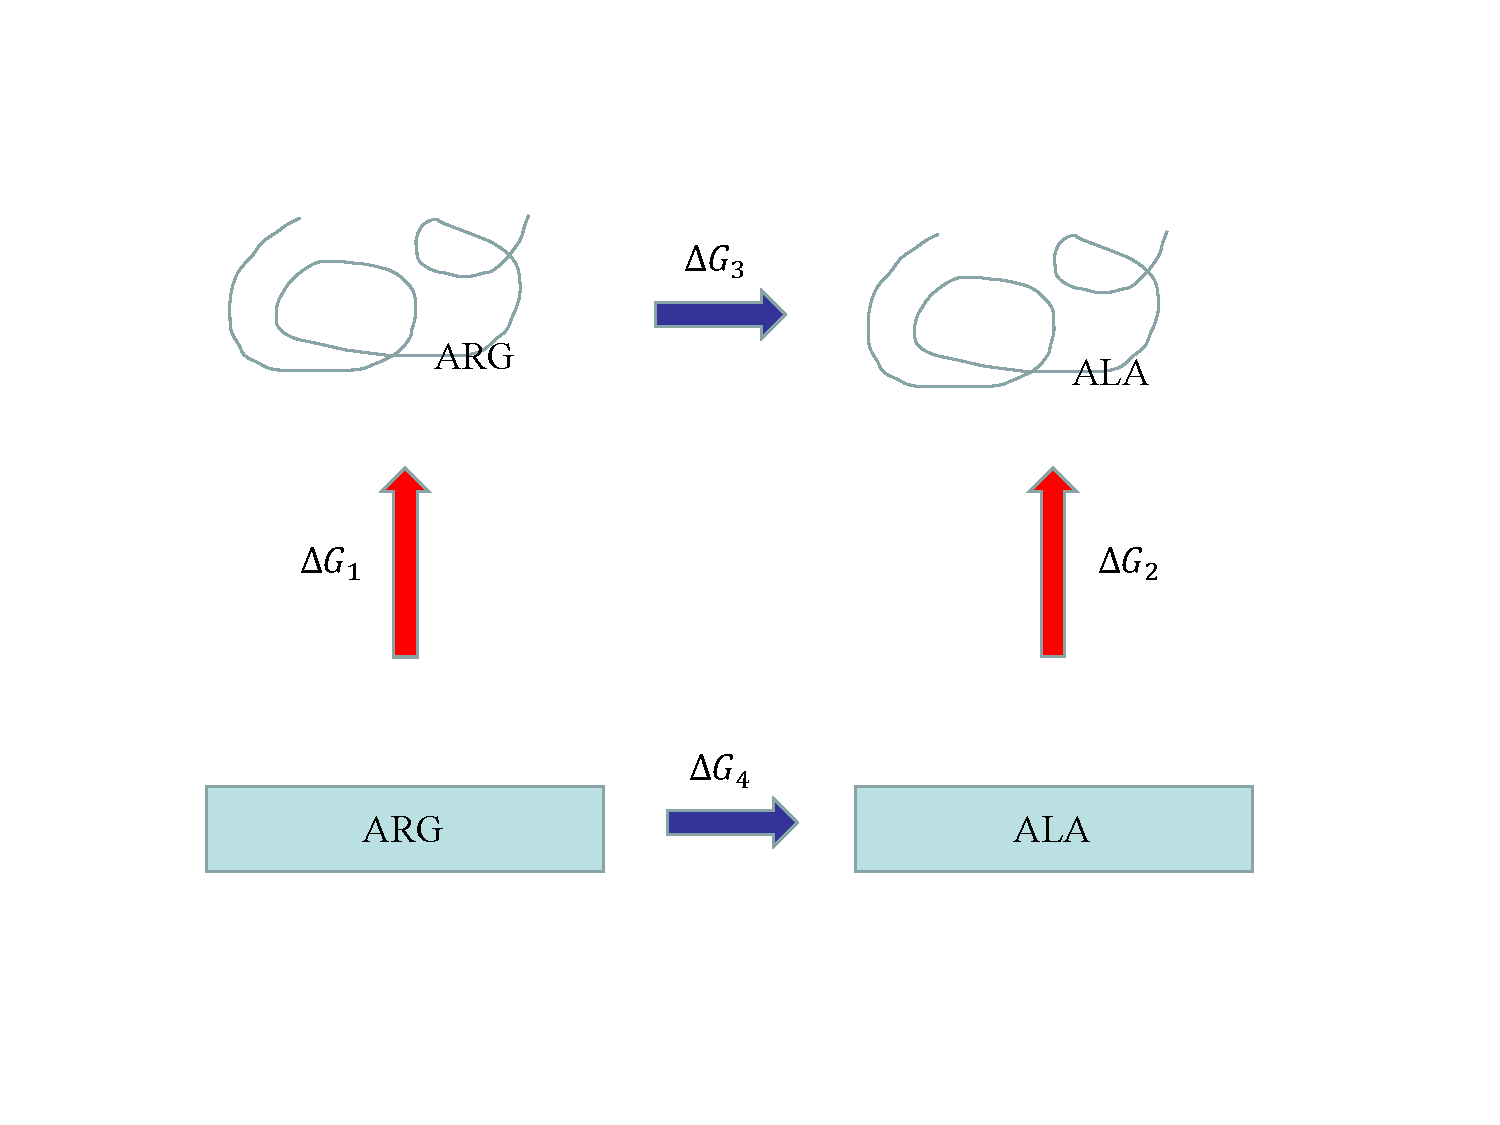
\includegraphics[width=\linewidth]{thermodynamic_cycle.pdf}
    \caption{the thermodynamic cycle used in this study}
    \label{cycle}
\end{figure}
Introduction to Thermodynamic Cycle
\begin{equation}
    \Delta G_1+\Delta G_3=\Delta G_2 + \Delta G_4
\end{equation}    
\begin{equation}
\Delta\Delta G = \Delta G_2 - \Delta G_1 = \Delta G_3 - \Delta G_4
\end{equation}



\section{Some Results}
\subsection{R120A}
\subsubsection{Folded State}
just test
\begin{figure}[h]
    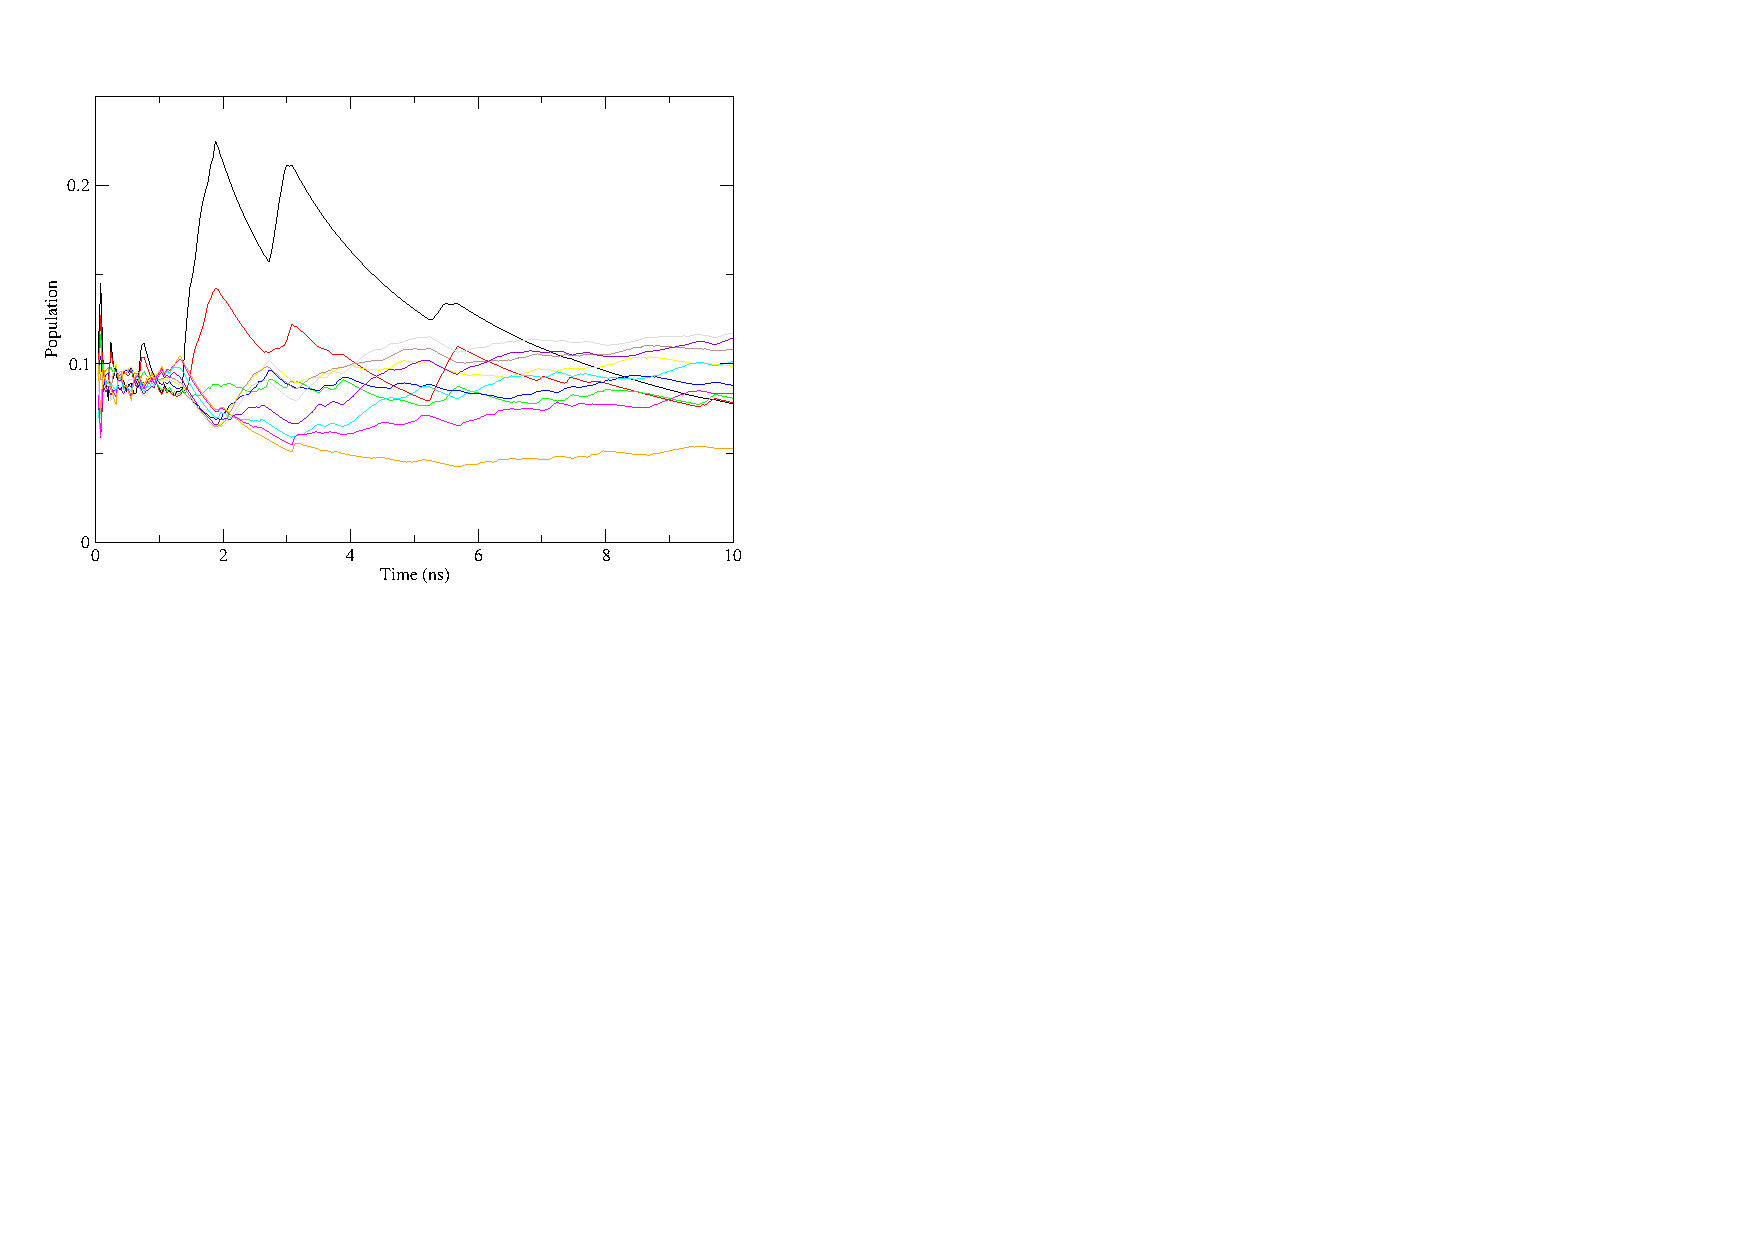
\includegraphics[width=\linewidth]{r120a_folded_pop.pdf}
    \caption{For R120A simuulation, the popolation on each state}
    \label{r120apop}
\end{figure}

\subsubsection{Linear State}

\subsection{R120I}
\subsubsection{Folded State}
just test
\begin{figure}[h]
    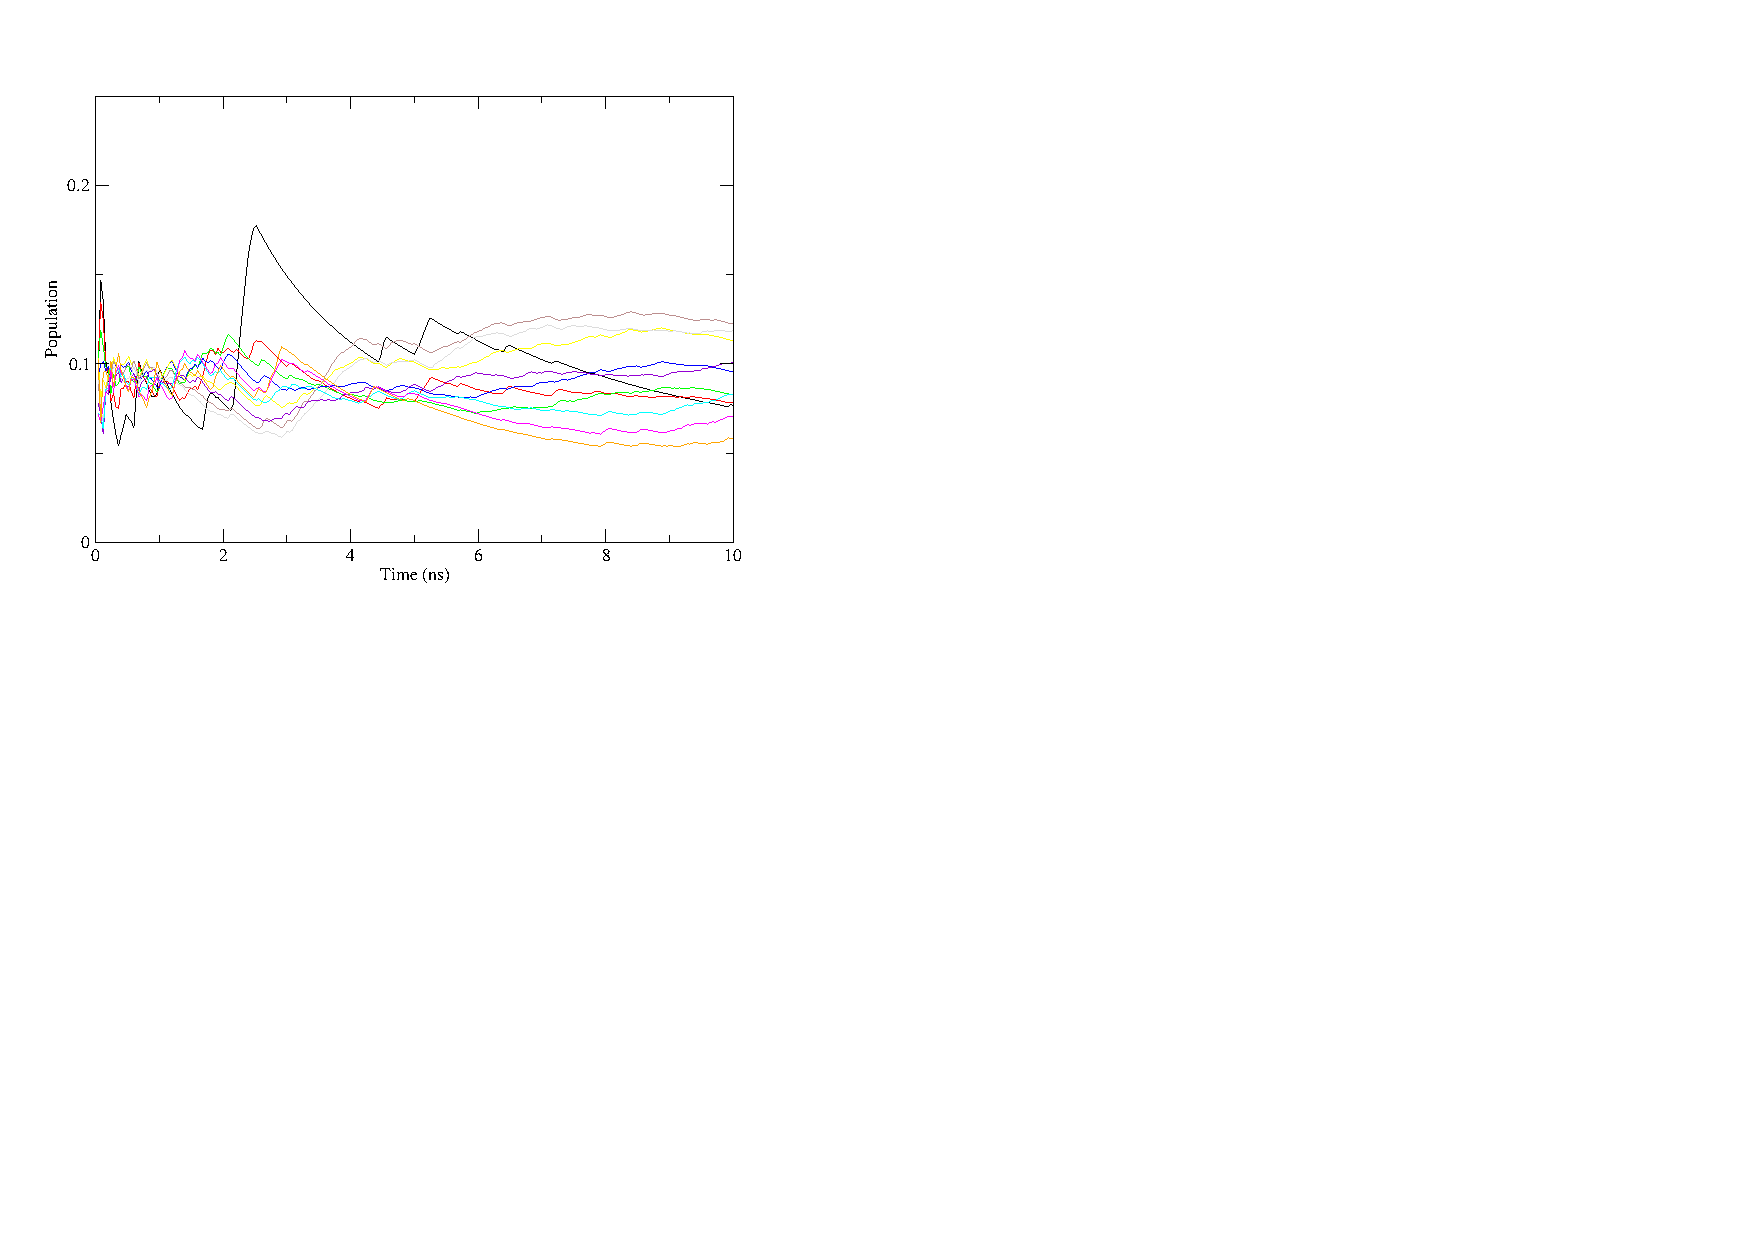
\includegraphics[width=\linewidth]{r120i_folded_pop.pdf}
    \caption{For R120I simulation, the popolation on each state}
    \label{r120ipop}
\end{figure}
\subsubsection{Linear State}

\subsection{R120L}
\subsubsection{Folded State}
just test
\begin{figure}[h]
    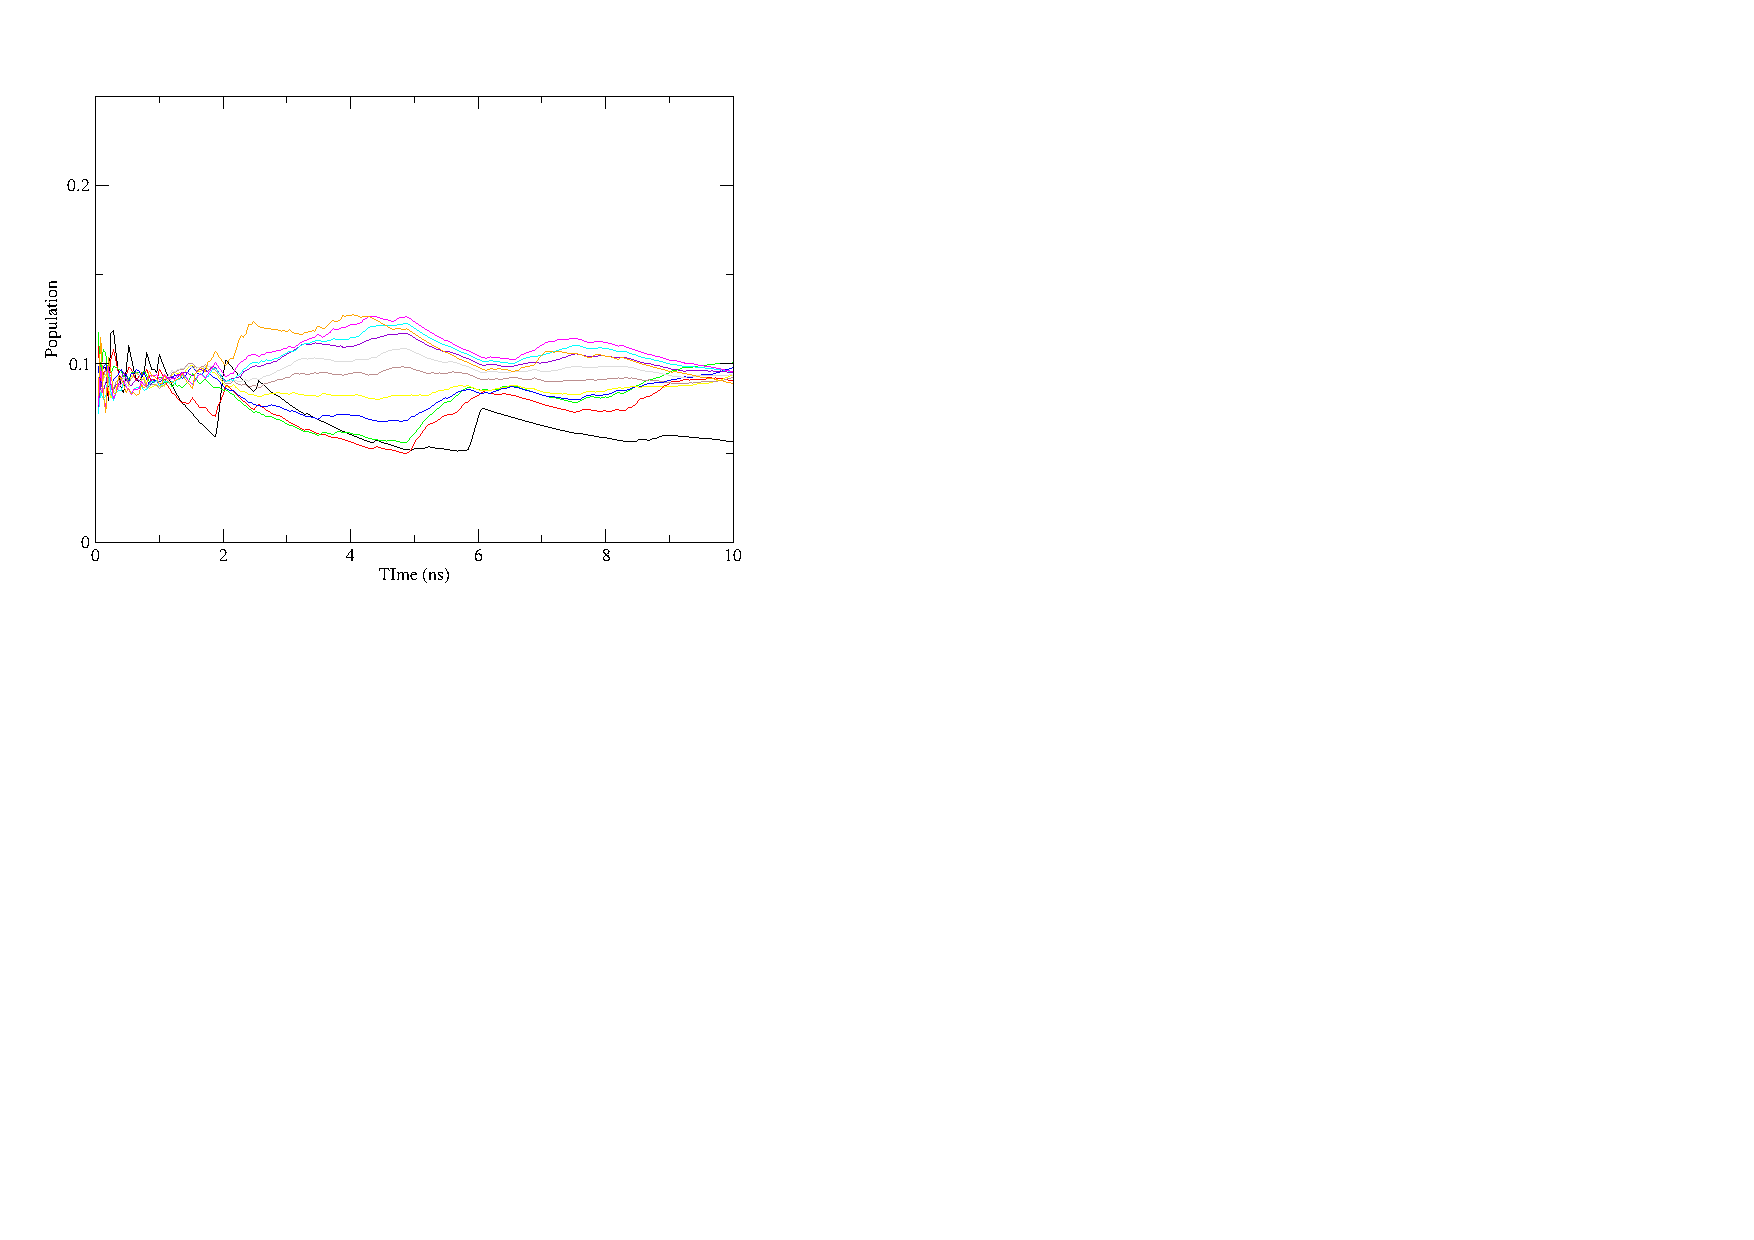
\includegraphics[width=\linewidth]{r120l_folded_pop.pdf}
    \caption{For R120L simulation, the popolation on each state}
    \label{r120lpop}
\end{figure}
\subsubsection{Linear State}

\subsection{R120Y}
\subsubsection{Folded State}
just test
\begin{figure}[h]
    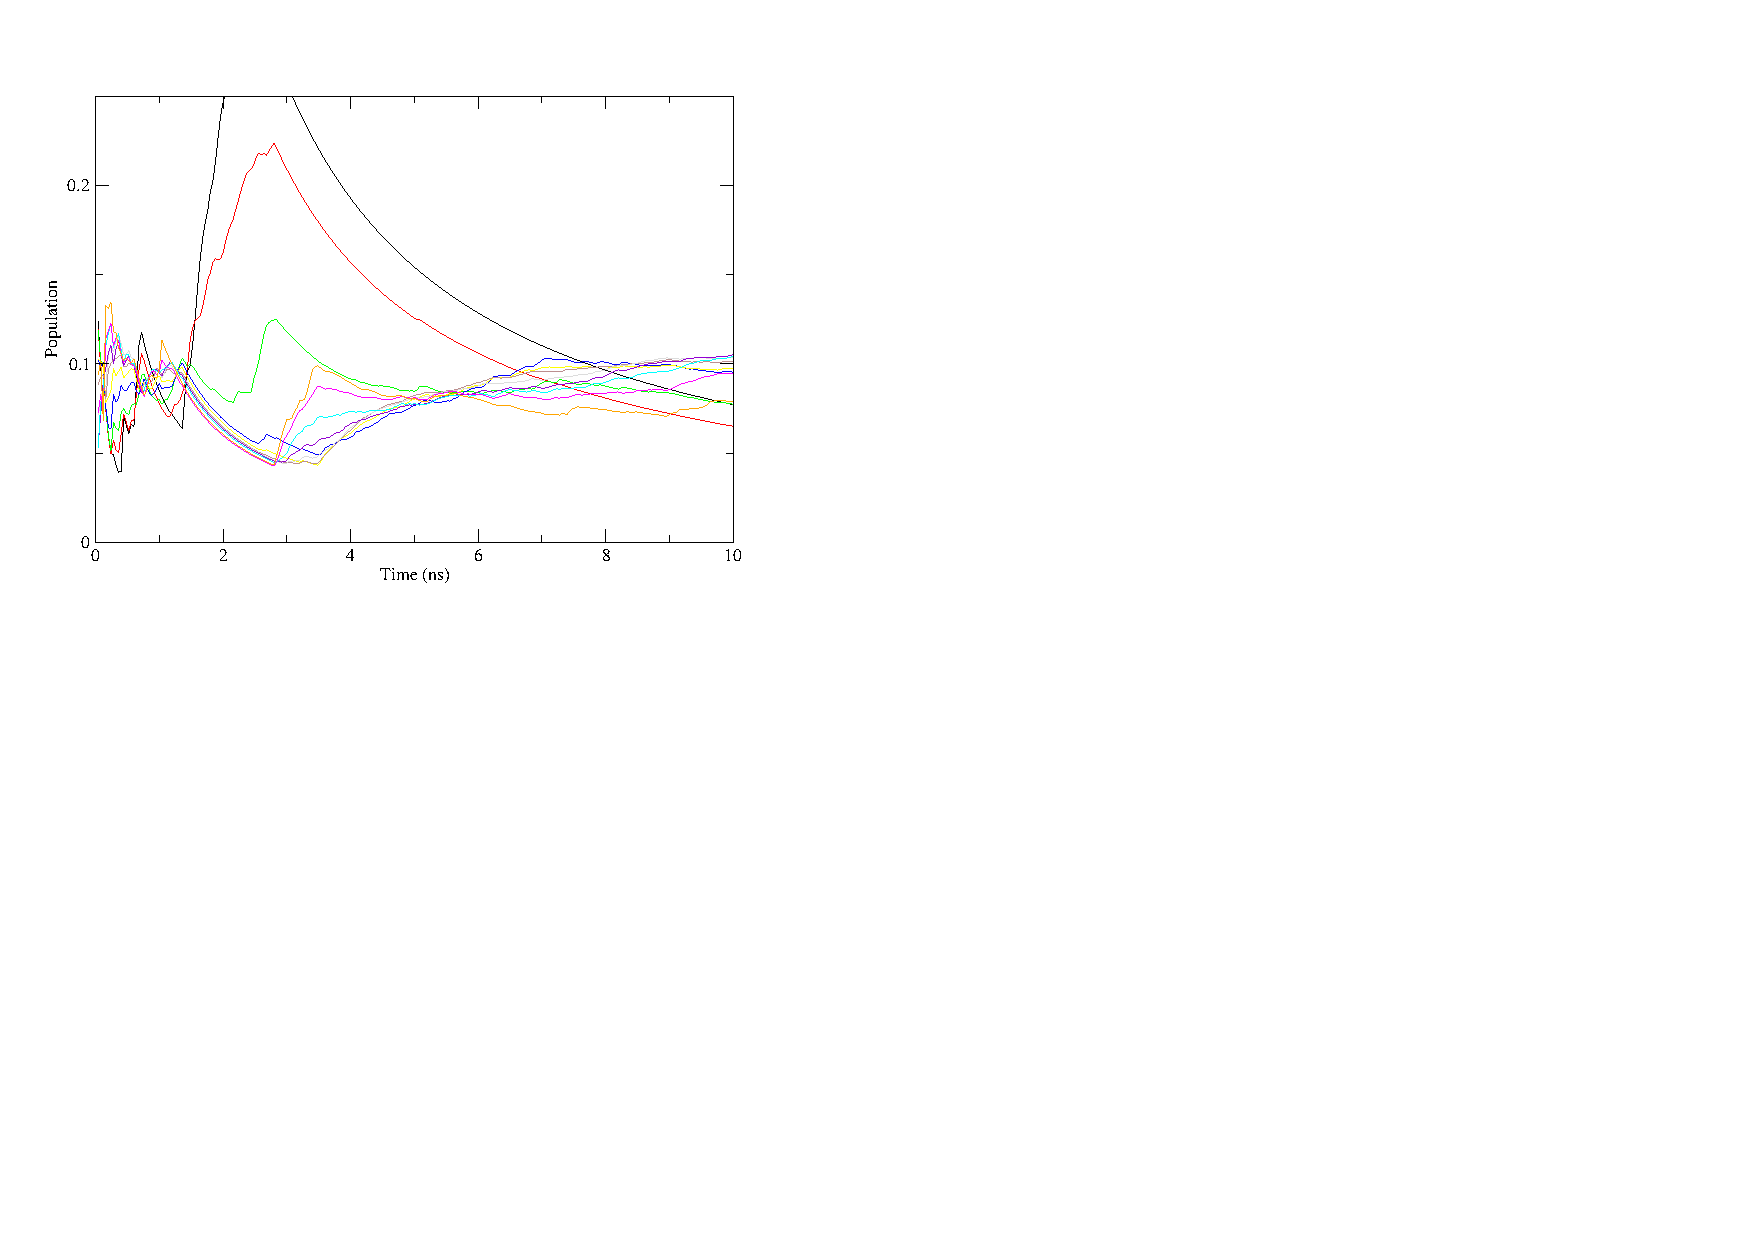
\includegraphics[width=\linewidth]{r120y_folded_pop.pdf}
    \caption{For R120Y simulation, the popolation on each state}
    \label{r120ypop}
\end{figure}
\subsubsection{Linear State}

\subsection{R120W}
\subsubsection{Folded State}
just test
\begin{figure}[h]
    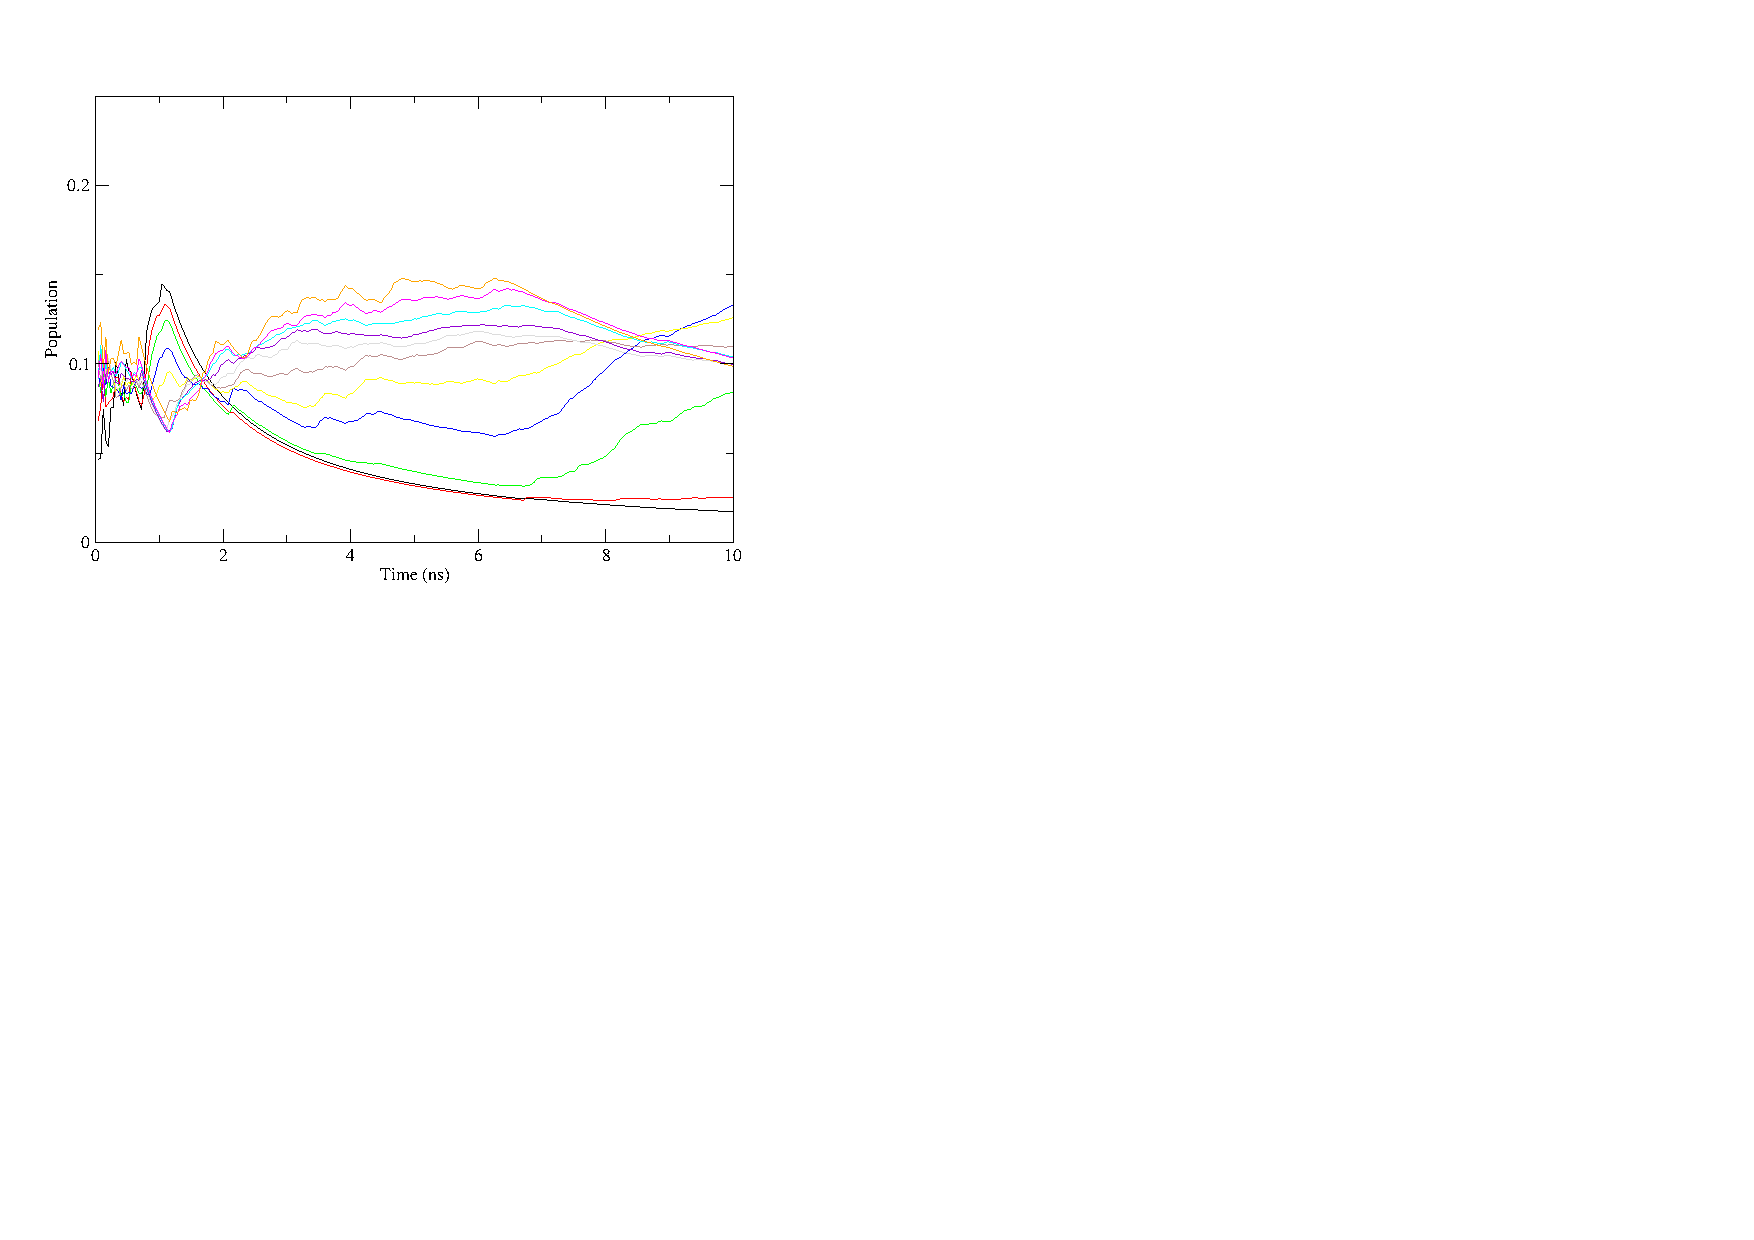
\includegraphics[width=\linewidth]{r120w_folded_pop.pdf}
    \caption{For R120W simulation, the popolation on each state}
    \label{r120wpop}
\end{figure}
\subsubsection{Linear State}

\subsection{R120F}
\subsubsection{Folded State}
just test
\begin{figure}[h]
    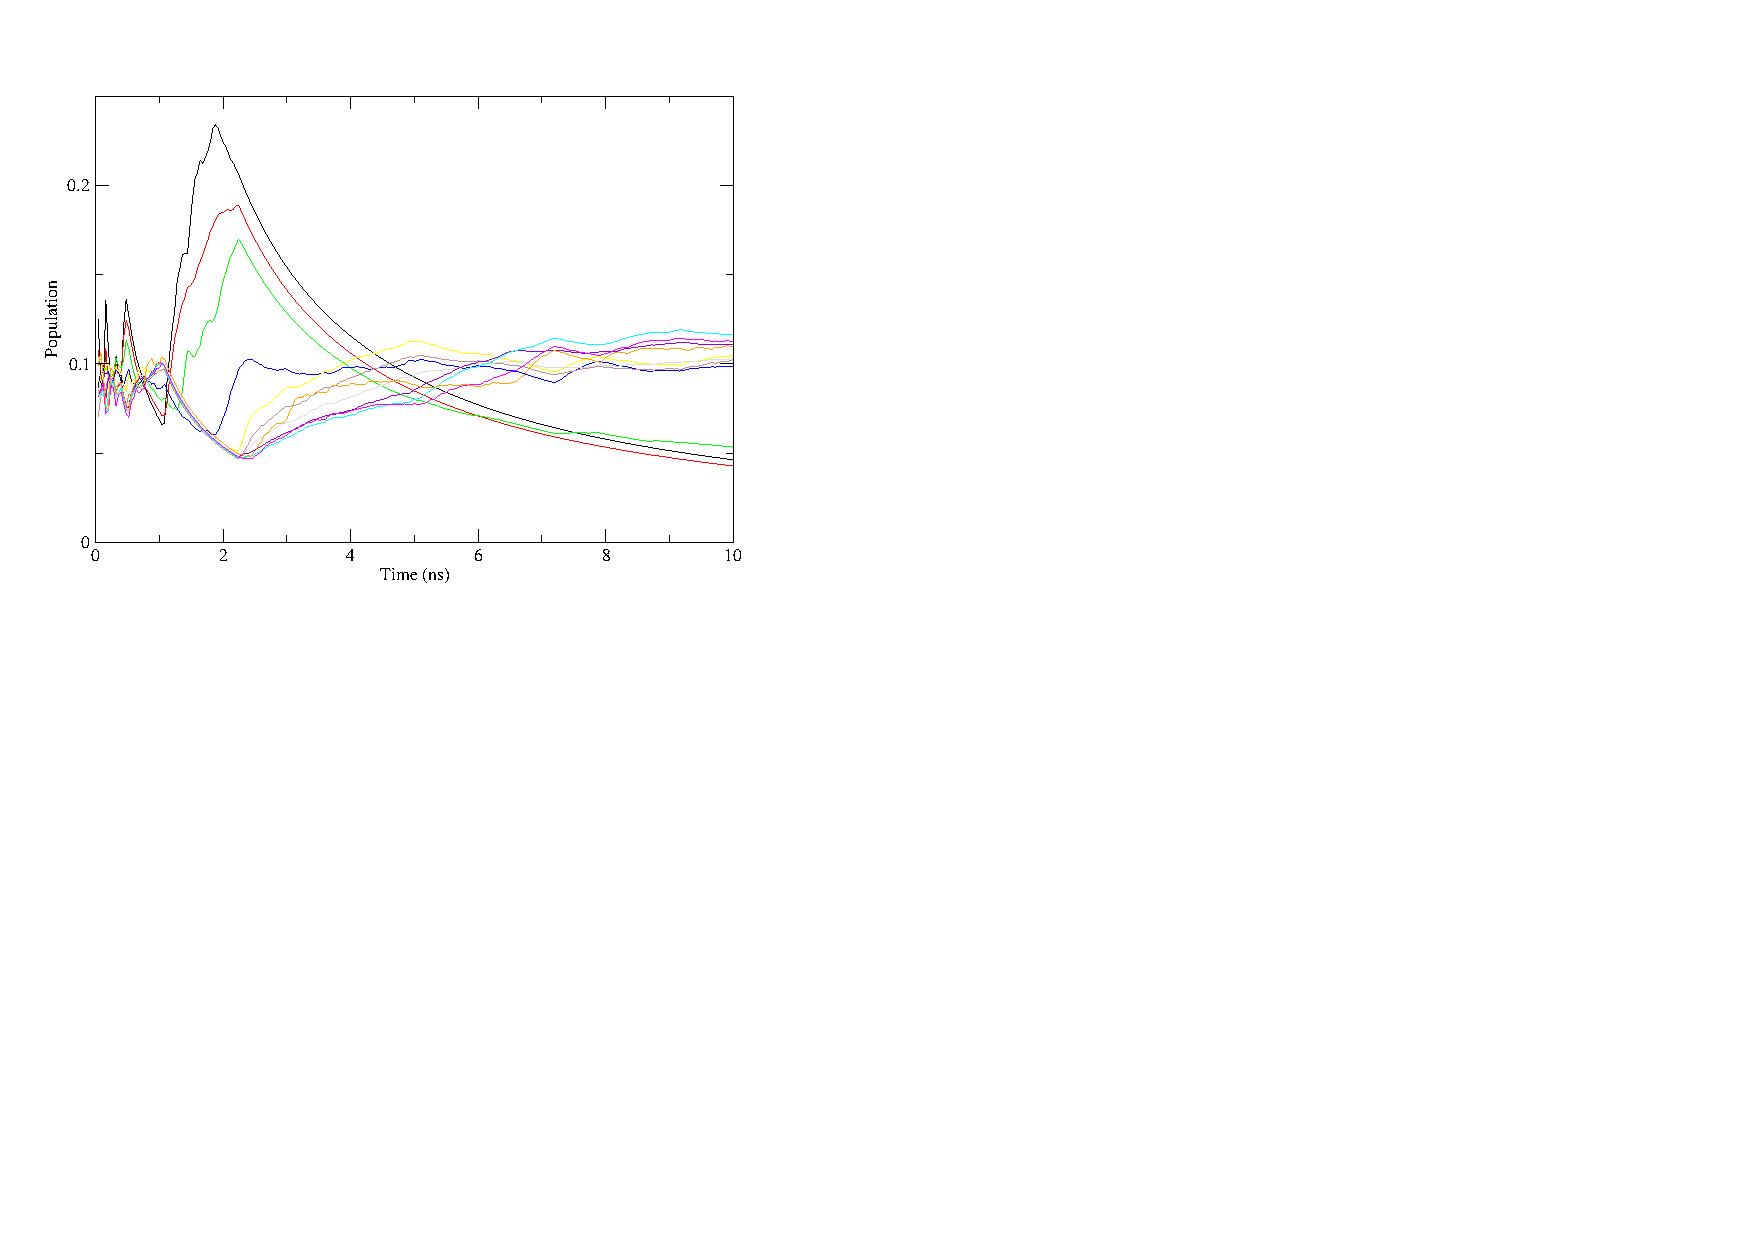
\includegraphics[width=\linewidth]{r120f_folded_pop.pdf}
    \caption{For R120F simulation, the popolation on each state}
    \label{r120fpop}
\end{figure}
\subsubsection{Linear State}

\subsection{R120Q}
\subsubsection{Folded State}
just test
\begin{figure}[h]
    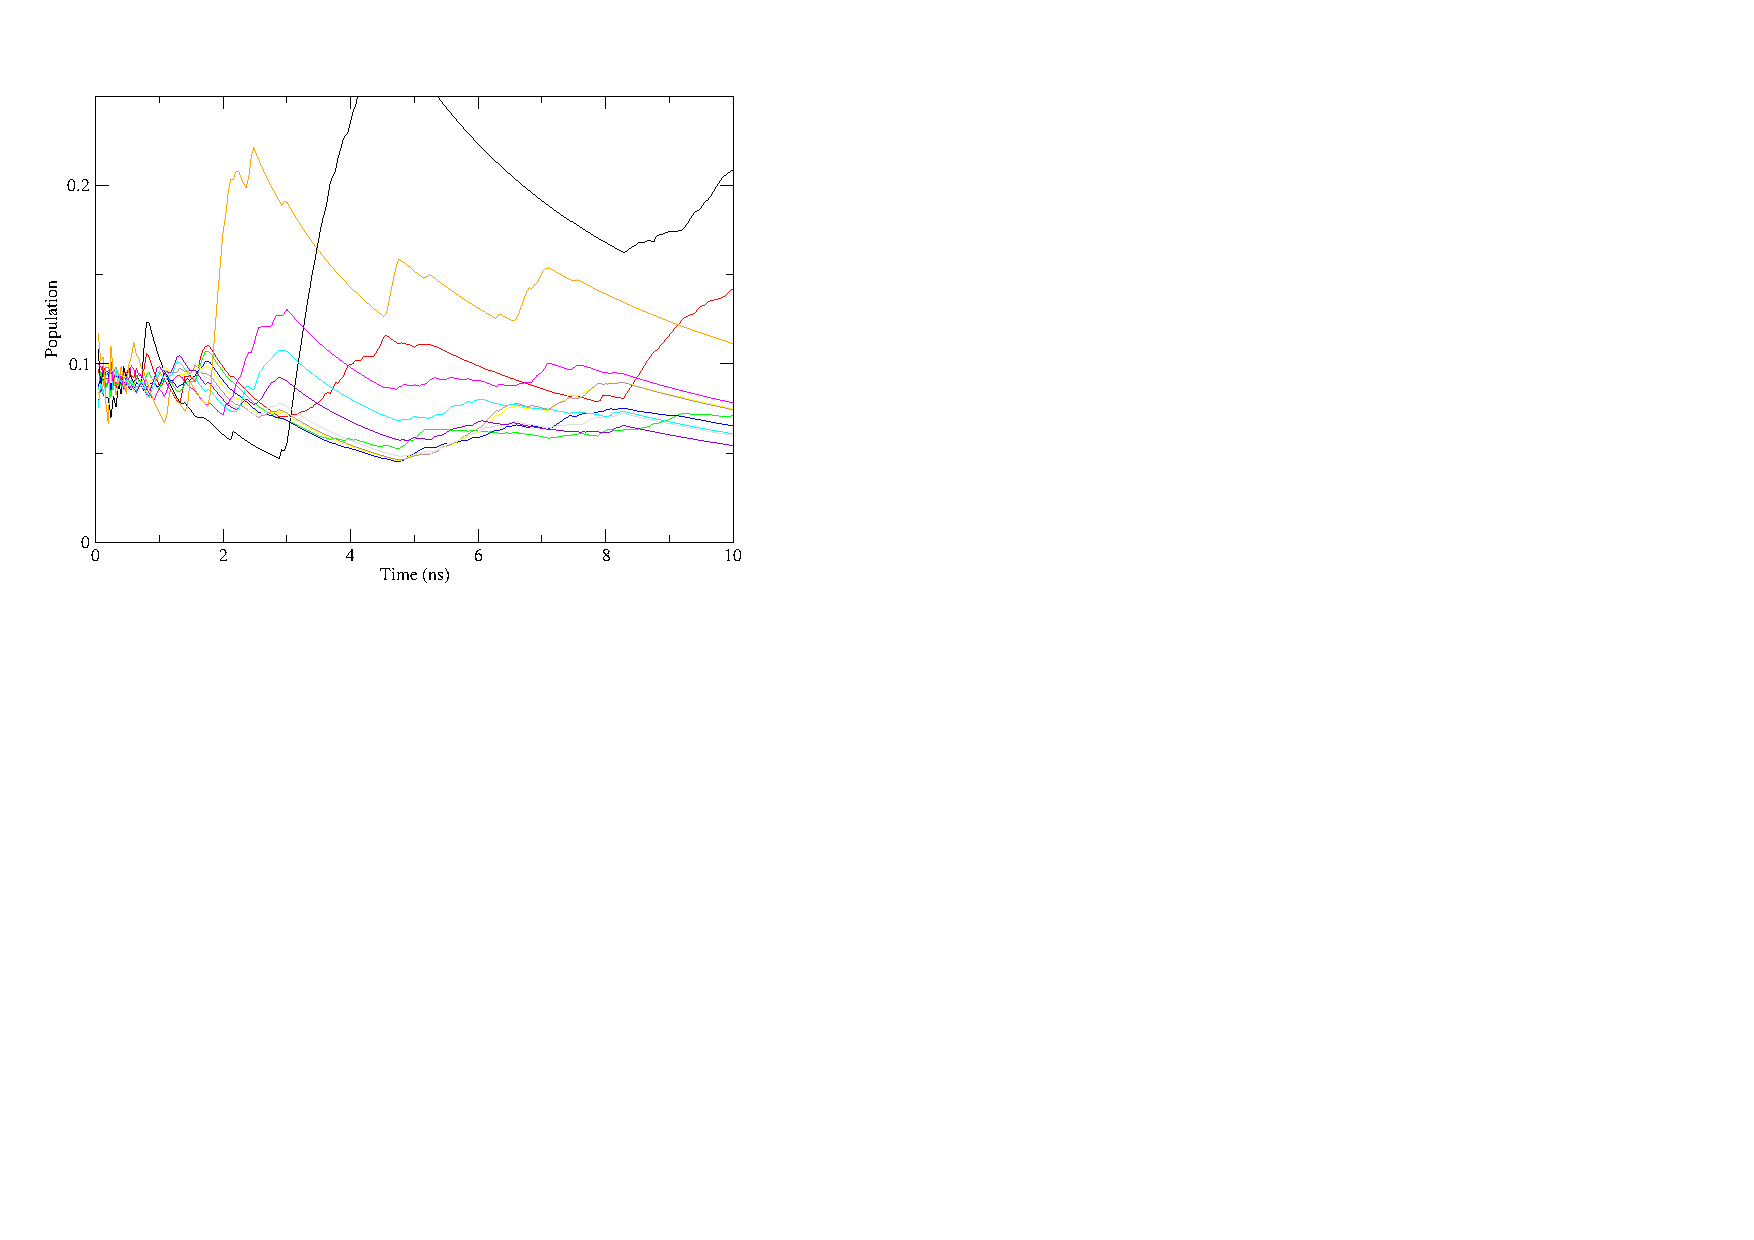
\includegraphics[width=\linewidth]{r120q_folded_pop.pdf}
    \caption{For R120Q simulation, the popolation on each state}
    \label{r120qpop}
\end{figure}
\subsubsection{Linear State}

\subsection{R120K}
\subsubsection{Folded State}
just test
\begin{figure}[h]
    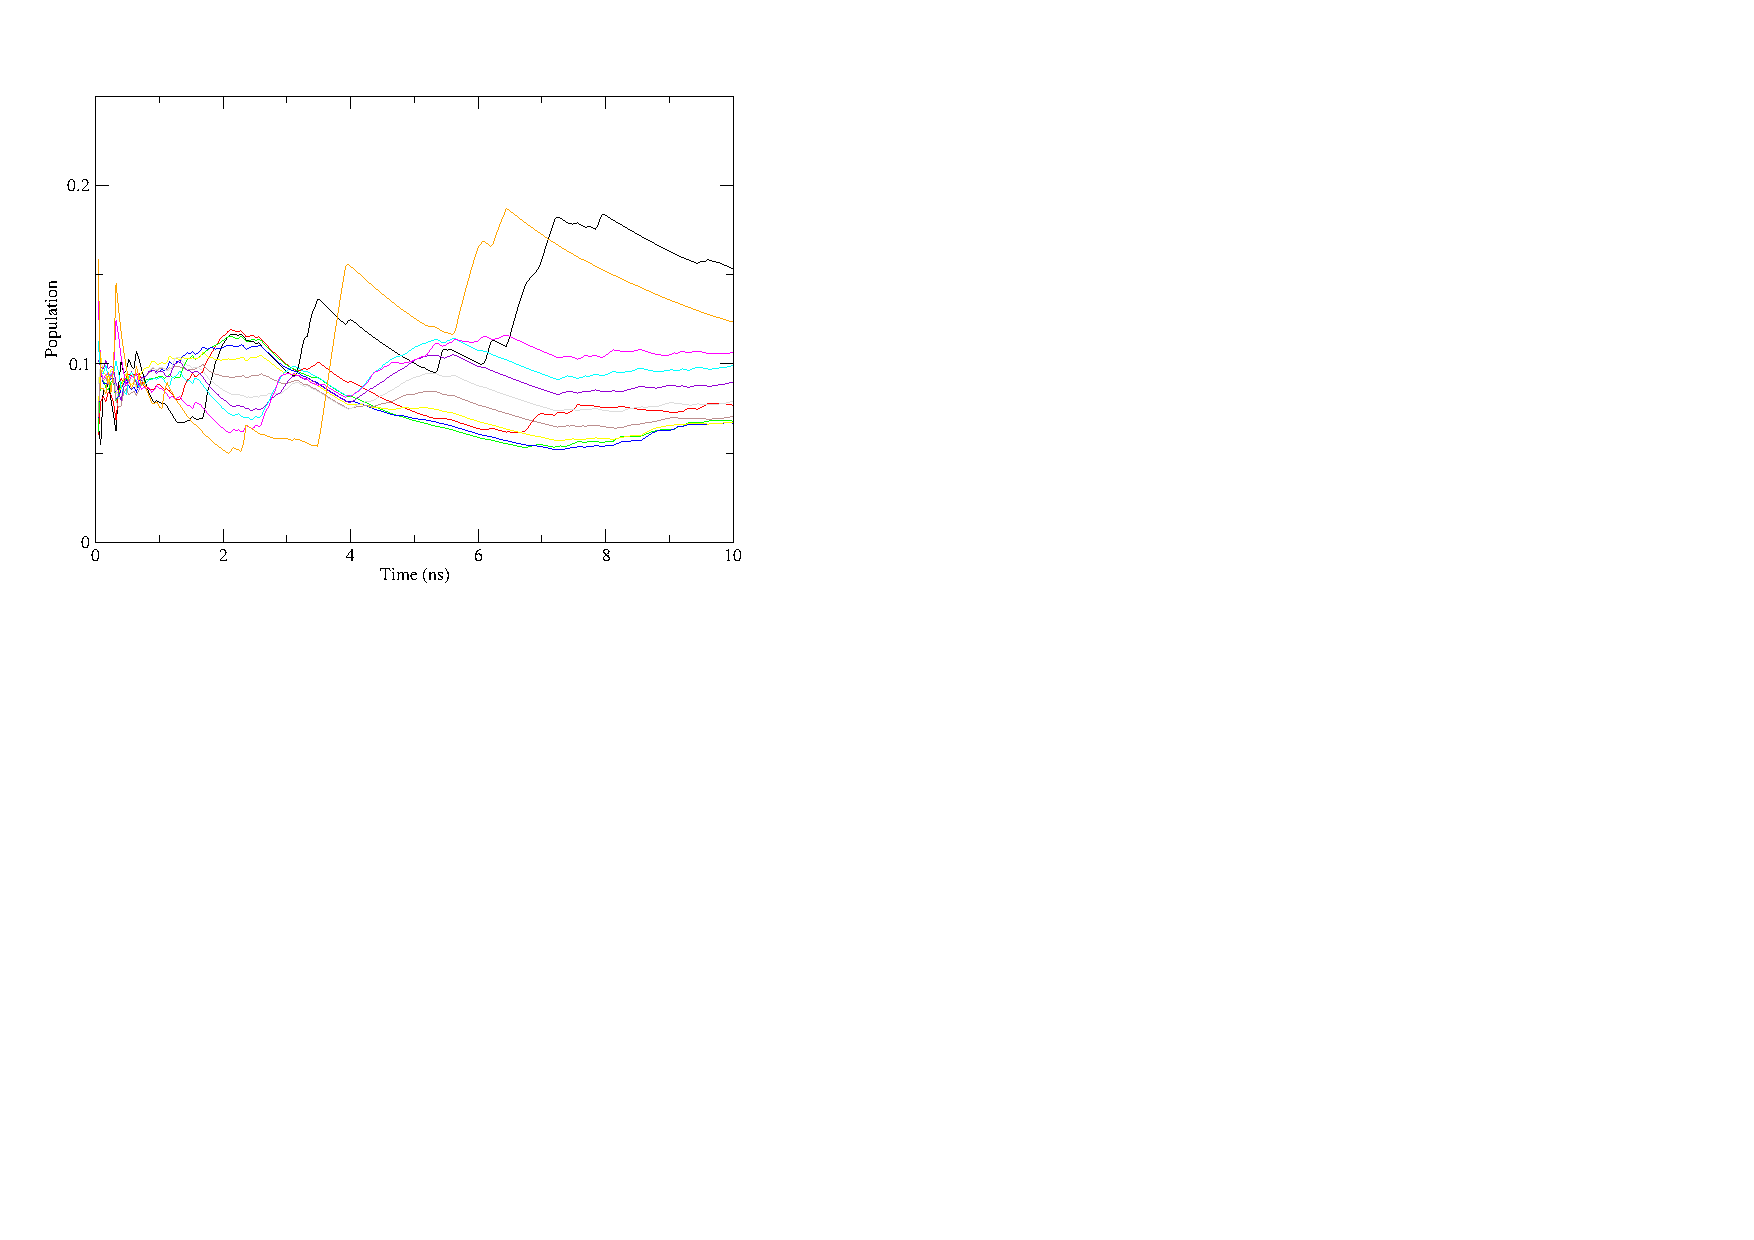
\includegraphics[width=\linewidth]{r120k_folded_pop.pdf}
    \caption{For R120K simulation, the popolation on each state}
    \label{r120kpop}
\end{figure}
\subsubsection{Linear State}

\subsection{Results}
\paragraph{results}
For R120F:$\Delta\Delta G=-4.99 kcal/mol$
\\
For R120F:$\Delta\Delta G=-4.99 kcal/mol$
\\
For R120A:$\Delta\Delta G=-1.84 kcal/mol$
\\
For R120I:$\Delta\Delta G=-2.74 kcal/mol$
\\
For R120L:$\Delta\Delta G=-3.69 kcal/mol$
\\
For R120K:$\Delta\Delta G=+0.62 kcal/mol$
\\
For R120Q:$\Delta\Delta G=+0.75 kcal/mol$
\\
For R120Y:$\Delta\Delta G=-4.53 kcal/mol$
\\
For R120W:$\Delta\Delta G=-7.89 kcal/mol$
\\
For K35W:$\Delta\Delta G=+1.85 kcal/mol$
\\
For K64R:$\Delta\Delta G=+0.70 kcal/mol$
\\
For K64S:$\Delta\Delta G=-1.51 kcal/mol$
\\
For V69I:$\Delta\Delta G=-0.75 kcal/mol$
\\
For V69L:$\Delta\Delta G=+0.03 kcal/mol$
\\
For K35I:$\Delta\Delta G=-1.29 kcal/mol$
\\
For K35V:$\Delta\Delta G=+0.28 kcal/mol$
\\
For K35L:$\Delta\Delta G=-0.03 kcal/mol$
\\
For K35L:$\Delta\Delta G=-0.03 kcal/mol$
\\
For L72I:$\Delta\Delta G=+0.28 kcal/mol$
\\
For Y45Q:$\Delta\Delta G=+1.80 kcal/mol$
\\
For Y45L:$\Delta\Delta G=+2.07 kcal/mol$
\\
For T37H:$\Delta\Delta G=-0.06 kcal/mol$
\\
For T37K:$\Delta\Delta G=-2.05 kcal/mol$
\\
For T41Q:$\Delta\Delta G=+1.77 kcal/mol$
\\
For T41E:$\Delta\Delta G=+2.29 kcal/mol$
\\
For F42Y:$\Delta\Delta G=+1.93 kcal/mol$
\\
For F42L:$\Delta\Delta G=+1.23 kcal/mol$
\\
\end{document}